\documentclass{report}
\usepackage{fancyhdr}
\usepackage{multicol}
\usepackage[italian]{babel}
\usepackage{imakeidx} % Indice analitico
\usepackage[a4paper]{geometry}


\usepackage{xcolor}
\usepackage{booktabs} %Gestione tabelle con \toprule
\usepackage{graphicx}

\usepackage{cookingsymbols}
\usepackage{hyperref}

\raggedcolumns
\setlength{\multicolsep}{0pt}
\setlength{\columnseprule}{1pt}

\makeindex[title=Indice degli ingredienti,intoc]
\makeatletter

\newif\if@mainmatter \@mainmattertrue

%% Borrowed from book.cls
\newcommand\frontmatter{%
    \cleardoublepage
  \@mainmatterfalse
  \pagenumbering{roman}}
\newcommand\mainmatter{%
    \cleardoublepage
  \@mainmattertrue
  \pagenumbering{arabic}}
\makeatother

% Your "recipes.sty" package starts here:
%% Thanks to alephzero for the excellent start:

\newcommand{\recipe}[2][]{%
    \newpage
    \lhead{\leftmark} % Titolo del capitolo nell'header
    \chead{}%
    \rhead{}%
    \lfoot{}%
    \rfoot{}%
    \section{#2}%

    \if###1##%
    \else
        \begin{center}
            \parbox{0.75\linewidth}{\raggedright\itshape#1}%
        \end{center}
    \fi
}
\newcommand{\autore}[1]{%
    \rhead{ Dal ricettario di: \textbf{#1}}}

%% Optional arguments for alternate names for these:
\newcommand{\serves}[1]{%
	    \vspace{15px}
	    \Fork\Dish\Knife \> #1 \>
    %\chead{#1 #2}
}
\newcommand{\preptime}[1]{%
	\Gloves \> #1 \>
	%\lfoot{#1 #2}%
}
\newcommand{\cooktime}[2][\Oven]{%
	\Gasstove \> #2 \>
	% \rfoot{#1: #2}%
}


\newcommand{\temp}[1]{%
    $#1^\circ$C}

%% Optional argument is the width of the graphic, default = 1in
\newcommand{\showit}[3][1in]{%
    \begin{center}
        \bigskip
            \includegraphics[width=#1]{#2}%
            \par
            \medskip
            \emph{#3}
            \par
        \end{center}%
    }

%% Optional argument for a  heading within the ingredients section
\newcommand{\ingredients}[1][]{%
    \if###1##%
    \vspace{15px} %Spazio sopra al titolo ingredienti
    \newline
        {\color{red}\Large\textbf{Ingredienti}}%
    \else
        \emph{#1}%
    \fi
}

%% Use \obeylines to minimize markup
\newenvironment{ingreds}{%
    \parindent0pt
    \noindent
    \ingredients
    \par
    \smallskip
    \begin{multicols}{2}
    \leftskip1em
    \rightskip0pt plus 3em
    \parskip=0.25em
    \obeylines
    \everypar={\hangindent2em}
}{%
    \end{multicols}%
    \medskip
}

%\newcounter{stepnum}

%% Optional argument for an italicized pre-step
%% Also use obeylines to minimize markup here as well
\newenvironment{method}[1][]{%
%    \setcounter{stepnum}{0}
    \vspace{15px}
    \noindent
    {\color{red}\Large\textbf{Preparazione}}%
    \par
    \par
    \smallskip
%    \if###1##%
%    \else
%        \noindent
%        \emph{#1}
%        \par
%    \fi
    \begingroup
    \parindent0pt
    \parskip0.25em
% La riga seguente è l'indentazione del testo della ricetta
%        \leftskip2em
% La riga seguente numera i passaggi della ricetta
%    \everypar={\llap{\stepcounter{stepnum}\hbox to2em{\thestepnum.\hfill}}}
}{%
    \par
    \endgroup}

\pagestyle{fancy}
% End of "recipes.sty"30



\begin{document}
\title{Appunti di cucina}
\author{AA.VV.}

\maketitle
\frontmatter
\tableofcontents

\mainmatter
\chapter*{Introduzione}

In questo testo sono raccolte le mie ricette preferite e quelle della mia famiglia. Alcune ricette sono state elaborate da me, altre, trovate sulla rete, su libri o riferite da amici, sono state adattate al mio gusto personale, alle mie esigenze, ai prodotti che utilizzo abitualmente in cucina e alle attrezzature di cui dispongo.

Se le ricette sono state prese da fonti diverse nelle prime righe del testo viene indicata la fonte alla quale si rimanda per approfondimento o per la licenza di utilizzo.

Tutte queste ricette sono state provate e sono state inserite qui perché mi sono piaciute e ho ritenuto valesse la pena ricordarle. Per questo motivo il presente testo non è un libro di ricette ma è il mio quaderno di \emph{Appunti di cucina}.

%\section{Simboli utilizzati nel testo}
In questo testo vengono utilizzati alcuni simboli per indicare i parametri della ricetta. \Fork\Dish\Knife \> Indica il numero di porzioni. \Gloves \> indica il tempo di preparazione della ricetta. \Gasstove \> indica il tempo di cottura.

\section{Appunti sulle temperature di cottura al cuore}
Conoscere la temperatura di cottura al cuore di un alimento è utile per poter replicare le ricette senza possibilità di errore e per garantire sempre il miglior risultato possibile secondo il proprio gusto personale.

La tabella \ref{temperature-al-cuore} è stata elaborata sulla base delle mie preferenze facendo prove con valori diversi, e annotando quelle che fornivano a mio parere un risultato ottimale.



\begin{table}
\begin{tabular}{llp{0.6\textwidth}}
\toprule
Alimento				&	Temp(°C)		&		Note		\\
\midrule
Hamburger			& 	62°C 		& Ideale per una cottura media\\
Arista di maiale	& 	71°C 		& Temperatura adatta per il maiale in genere che risulterà sicuro e succoso. Non è adatta per cotture di tagli duri tipo costine o pulled pork. \\
Pollo ripieno 		& 	71°C 		& Temperatura ideale per qualunque volatile ripieno\\
Polpettone di manzo	&	75°C 		& Temperatura ideale se si aggiunge pane ammollato nel latte, altrimenti meglio abbassare un po' la temperatura\\
\bottomrule
\end{tabular}
\caption{Temperature di cottura al cuore dell'alimento ottimali secondo il mio gusto personale.}\label{temperature-al-cuore}

\end{table}

\section{Appunti di cottura a bassa temperatura (CBT)}
La cottura a bassa temperatura (CBT) è una tecnica che consiste nella cottura di un alimento imbustato sotto vuoto in bagno termostatico ad una temperatura che in genere varia dai \temp{52} agli \temp{80}.

I tempi di cottura con questa tecnica variano da un minimo di 30 minuti, ma possono arrivare anche alle 36-48 ore. In questa tecnica di cottura il tempo risulta spesso utile a sciogliere il collagene e a rendere teneri anche tagli di carne particolarmente duri, tuttavia, poiché il parametro delle temperatura è costate, spesso variare il tempo non comporta grandi cambiamenti nel risultato finale. Nella tabella \ref{temperature-cbt} ho sintetizzato i parametri di cottura che preferisco.

Se sei interessato a questa tecnica di cottura e stai leggendo questo testo, ti consiglio di leggere guide più esaustive soprattutto per chiarire alcuni aspetti legati alla sicurezza alimentare.

\begin{table}
\begin{tabular}{lllp{0.5\textwidth}}
\toprule
Alimento				&	Temp			&	Tempo	&	Note	\\
\midrule
Uovo					&	\temp{63}	&	1 ora	&	Simile all'uovo in camicia \\
Costata bovino		&	\temp{52}	&	2-3 ore	&	Per una cottura al sangue perfetta \\
Vitello tonnato		&	\temp{58}	&	4-5 ore &	\\
Costine di maiale	&	\temp{62}	&	12 ore	&	Poi rifinite in forno \\
Roast beef			&	\temp{58}	&	4-5 ore	&	Poi rifinito in padella in ferro \\
Filetti di sgombro	&	\temp{60}	&	40 minuti \\
\bottomrule
\end{tabular}
\caption{Temperature e tempi di cottura CBT per gli alimenti che cucino più spesso.}\label{temperature-cbt}
\end{table}



\newpage
\chapter{Pane e lievitati}
\recipe[Non so dove mia mamma abbia scoperto questa ricetta. Fare i crackers in casa è facilissimo e sono anche molto buoni.]{Crackers al sesamo}
\serves{4}
\preptime{1 ora}
\cooktime[Cottura]{30 minuti}
\autore{Max (Nonna Giuli)}
\begin{ingreds}
	280g di \index{farina}
	50g di acqua
	50g di olio evo
	100g di vino bianco
	50g di sesamo
	5g di sale
\end{ingreds}

\begin{method}
	Metti la farina, il sale, il sesamo nella bull della planetaria e mescola. Aggiungi la parte liquida e impasta leggermente con la foglia. Fai riposare la pasta per 20 minuti coperta con una pellicola.
	Tira la pasta con la macchinetta fino alla misura 3 senza ripiegare. Taglia i crackers e mettili sulla leccarda ricoperta di carta da forno.

	Cuoci in forno ventilato a \temp{180} per 25/30 minuti.
\end {method}


\recipe[Questa ricetta mi è stata insegnata ad un corso di cucina. Prima facevo i panini con una ricetta molto più lunga e complicata. Con questa ricetta il risultatto non è molto diverso e si perde meno tempo.]{Panini da hamburgher veloci}\label{panini-hamburger}
\serves{8}
\preptime{2 ore e 30}
\cooktime[Cottura]{30 minuti}
\autore{Max}
\begin{ingreds}
	500g di farina 0
	250g di acqua fredda
	30g di strutto
	10g di sale
	25g di lievito
\end{ingreds}

\begin{method}
	Metti tutti gli ingredienti nella planetaria e impasta per 10 minuti.

	Dai un paio di pieghe alla pasta e forma le palline. Per mini hamburgher fai palline da 30g per hamburgher tradizionali fai palline da 120g. Questa operazione si chiama pirlatura. Si tratta di richiudere la pasta su se stessa come un sacchetto in modo che la gabbia glutinica intrappoli le bolle d'aria che si sviluppano durante la lievitazione.

	Fai lievitare fino al raddoppio del volume. Servirà circa 1 ora e 30 minuti, ma questo tempo può variare in base alla temperatura e alla quantità di lievito che decidi di utilizzare.
	
	Quando i panini sono lievitati, se vuoi, puoi spennellare la superfice con tuorlo d'uovo e acqua o latte e successivamente cospargere semi si sesamo o altri semi. Questa operazione, oltre a rendere i panini più belli, conferirà ai panini una nota profumata interessante.

	Cuoci i panini in forno ventilato a \temp{190} per 15 minuti.

\end{method}

\recipe[]{Pizza in teglia}
\serves{4}
\preptime{1 ora}
\cooktime[]{30 minuti}
\autore{Max}
%\vegetarian
%\freeze
\begin{ingreds}
	1kg farina 1 + manitoba
	40g olio e.v.o.
	20 sale
	10g lievito di birra secco
	800g acqua
%\columnbreak
%\ingredients[For the Crumble Mixture:]
\end{ingreds}

\begin{method}
\underline{Impasto a mano.} Il pomeriggio del giorno prima metti in una ciotola la farina e il lievito poi mescola. Aggiungi poco alla volta l'acqua fino a incorporarla tutta. Poi aggiungi il sale, l'olio e mescola con un cucchiaio. L'impasto rimarrà grumoso. Aspetta 15 minuti poi metti l'impasto sulla spianatoia infarinata e piega in 3, prima da una parte poi dall'altra. Ripeti queste pieghe 3 o 4 volte lasciando un tempo di riposo di 15 minuti fra una piega e la successiva.

\underline{Impasto con la planetaria} Se vuoi usare la planetaria, metti tutti gli ingredienti nella ciotola e impasta per 8 minuti a velocità medio alta con la foglia. Poi rimuovi la pasta dalla foglia e fai riposare per 10 minuti. Fai partire la planetaria alla velocità minima giusto il tempo di raccogliere la pasta poi fai altri 10 minuti di riposo e ripeti l'operazione. Trasferisci l'impasto sul piano in acciaio oliato e fai le pieghe, lasciando riposare la pasta 10 minuti fra una piega e la successiva.

Metti l'impasto già diviso in 2 in un contenitore ermetico unto e fai lievitare in frigo per tutta la notte.

Il giorno successivo togli l'impasto dal frigo alle 15:00 e lascia a temperatura ambiente. Dopo un paio d'ore stendi sulla leccarda oliata e fai lievitare per 2 o 3 ore. Cuoci in forno statico a \temp{250} mettendo la leccarda nel ripiano più basso per 10 minuti. Poi abbassa a \temp{230} per 10 minuti al centro del forno.




%\begin{table}[h]
%\begin{tabular}{lcc}
%\toprule
%	Ingredienti	&	Peso(g)	&	Peso(g)\\
%\midrule
%	Paprika		&	40	&	60	\\
%	Sale		&	33	&	50	\\
%	Zucchero	&	20	&	30	\\
%	Cumino		&	2	&	3	\\
%	Pepe		&	6	&	9	\\
%	Aglio		&	12	&	18	\\
%	Origano		&	2	&	3	\\
%\bottomrule
%\end{tabular}
%\end{table}

\end{method}

%\showit[1.25in]{example-image-b}{This is a picture}



\newpage
\chapter{Antipasti}
\recipe[Questa ricetta mi è stata insegnata ad un corso di cucina. La cottura sulla foglia di alloro e la panna acida rendono questa ricetta interessante.]{Mini hamburger di orata}
\serves{4}
\preptime{1 ora}
\cooktime{5 minuti}
\autore{Max}
\begin{ingreds}
	200g orata
	4 foglie di alloro
	1 pezzo di porro
	Pane da hamburgher (Vedi ricetta \ref{panini-hamburger})
	
\columnbreak
\ingredients[Per la panna acida:]
	1 cipolla
	1 bicchiere di aceto
	1 bicchiere di vino
	125g di panna fresca
\end{ingreds}

\begin{method}
Per prima cosa prepara la panna acida, se vuoi puoi farla anche il giorno prima conservandola in frigo. Fai stufare la cipolla tagliata a striscioline, poi aggiungi il vino e l'aceto e fai ridurre lentamente. Nel frattempo in un padellino fai ridurre la panna. Setaccia e spremi la cipolla. Aggiungila alla panna e fai riposare in frigorifero per qualche ora.

Sfiletta l'orata e prepara una tartare battuta a coltello. Con il coppapasta prepara dei mini hamburger serrandoli con mezza foglia di alloro sui due lati. Lascia riposare gli hamburger in frigorifero.

Taglia il porro a juilenne sottili, infarinalo e friggilo in olio di semi di girasole a \temp{170}.

Taglia il pane con il coppapasta che hai usato per preparare gli hamburger e fallo tostare in forno. Cuoci gli hamburger in una padella antiaderente senza esagerare con la cottura. Componi i panini con la panna acida, l'hamburger di orata al quale avrai tolto le foglie di alloro e il porro fritto. Puoi fermare i panini con uno stuzzicadente.
\end{method}
\subsection*{Note}
		Puoi sostituire l'orata con pesci simili: branzino, ricciola, pagello. Anche con il salmone non è mala, ma meno delicato.




\newpage
\chapter{Sale e preparazioni di base}
\recipe[]{Besciamella}\label{besciamella}
\serves{-}%<----Numero di porzioni
\preptime{15 minuti}%<---Tempo di preparazione
\cooktime[]{10 minuti}%<-----Tempo di cottura
\autore{Max}
\begin{ingreds}
	% Qui gli ingredienti uno sotto all'altro
	500g latte intero
	50g burro (anche meno)
	50g farina 00
	Noce moscata (o altri aromi)
	Sale

% Se vuoi aggiungere gli ingredienti per una preparazione
% specifica della ricetta usa questi 2 comandi
%\columnbreak
%\ingredients[Per il ripieno:]

\end{ingreds}

\begin{method}
Scalda il latte intero senza portarlo a bollore. Fai sciogliere il burro in una casseruola, aggiungi la farina e falla imbiondire mescolando con un cucchiaio di legno.

Aggiungi poco alla volta il latte, mescolando vigorosamente con una frusta per evitare la formazione di grumi.

Quando avrai versato tutto il latte riporta sul fuoco e cuoci per portare alla consistenza desiderata. Aggiungi la noce moscata o altri aromi e regola di sale.

\end{method}

\subsection*{Note}
La ricetta base della besciamella che si presta a diverse varianti (es. olio e.v.o. al posto del burro e brodo vegetale al posto del latte. Se dovessero formarsi dei grumi puoi frullare con un frullatore a immersione.

% Figura
%\showit[1.25in]{example-image-b}{This is a picture}



\recipe[]{Cipolle caramellate}
\serves{4}
\preptime{1 ora}
\cooktime[Cottura]{30 minuti}
\autore{Max}
%\vegetarian
%\freeze
\begin{ingreds}
	500g di cipolle rosse
	100g di zucchero
	30g di aceto
	un pizzico di sale
	olio e.v.o.
%\columnbreak
%\ingredients[For the Crumble Mixture:]

\end{ingreds}

\begin{method}
Taglia a metà le cipolle sbucciate e affettale, poi falle appassire in un tegame con un filo d'olio e un pizzico di sale.

Quando le cipolle iniziano a sfrigolare aggiungi lo zucchero e continua a cuocere a fuoco moderato. Quando sfrigola di nuovo aggiungi l'aceto per fissare il colore e dare il giusto grado di acidità utile per la conservazione in vaso.


%\begin{table}[h]
%\begin{tabular}{lcc}
%\toprule
%	Ingredienti	&	Peso(g)	&	Peso(g)\\
%\midrule
%	Paprika		&	40	&	60	\\
%	Sale		&	33	&	50	\\
%	Zucchero	&	20	&	30	\\
%	Cumino		&	2	&	3	\\
%	Pepe		&	6	&	9	\\
%	Aglio		&	12	&	18	\\
%	Origano		&	2	&	3	\\
%\bottomrule
%\end{tabular}
%\end{table}

\end{method}

%\showit[1.25in]{example-image-b}{This is a picture}



\recipe[]{Maionese}\label{maionese}
\serves{4}
\preptime{10 minuti}
\cooktime[Cottura]{3 minuti (versione pastorizzata)}
\autore{Max}
%\vegetarian
%\freeze
\begin{ingreds}
	1 uovo
	200ml di olio di semi di girasole
	un cucchiaino di senape
	un pizzico di sale
	un cucchiaio di limone
%\columnbreak
%\ingredients[For the Crumble Mixture:]

\end{ingreds}

\begin{method}
\underline{Versione rapida}. Metti tutti gli ingredienti ad esclusione del limone nel bicchiere del frullatore a immersione. Inserisci il frullatore a immersione fino al fondo del bicchiere poi azionalo alla massima potenza. Non muovere il frullatore fino a che non vedi la maionese che inizia a formarsi. A quel punto sali lentamente. Aggiungi il limone e continua a frullare per amalgamare gli ingredienti.

\underline{Versione pastorizzata}. Metti l'olio in un tegame e porta a \temp{121}. Metti gli altri ingredienti nel bicchiere del frullatore a immersione e frulla per amalgamare, poi aggiungi l'olio caldo a filo continuando a frullare fino ad ottenere una maionese soda. Lascia raffreddare prima di mangiare.



%\begin{table}[h]
%\begin{tabular}{lcc}
%\toprule
%	Ingredienti	&	Peso(g)	&	Peso(g)\\
%\midrule
%	Paprika		&	40	&	60	\\
%	Sale		&	33	&	50	\\
%	Zucchero	&	20	&	30	\\
%	Cumino		&	2	&	3	\\
%	Pepe		&	6	&	9	\\
%	Aglio		&	12	&	18	\\
%	Origano		&	2	&	3	\\
%\bottomrule
%\end{tabular}
%\end{table}

\end{method}

%\showit[1.25in]{example-image-b}{This is a picture}



\recipe[]{Rub: My Magic Dust}
\serves{-}
\preptime{5 minuti}
\cooktime[Cottura]{-}
\vegetarian
\begin{ingreds}
	Vedi tabella nella preparazione
%\columnbreak
%\ingredients[For the Crumble Mixture:]

\end{ingreds}

\begin{method}
Miscela tutti gli ingredienti e posiziona in un barattolo. Ogni tanto ricorda di scuotere il barattolo.
\begin{table}[h]
\begin{tabular}{lcc}
\toprule
	Ingredienti	&	Peso(g)	&	Peso(g)\\
\midrule
	Paprika		&	40	&	60	\\
	Sale		&	33	&	50	\\
	Zucchero	&	20	&	30	\\
	Cumino		&	2	&	3	\\
	Pepe		&	6	&	9	\\
	Aglio		&	12	&	18	\\
	Origano		&	2	&	3	\\
\bottomrule
\end{tabular}
\end{table}
\end{method}

%\showit[1.25in]{example-image-b}{This is a picture}



\recipe[]{Salsa BBQ all'abicocca}\label{salsa-bbq}
\serves{-}
\preptime{1 ora}
\cooktime{10 minuti}
\autore{Max}
\begin{ingreds}
	200g di doppio \index{concentrato di pomodoro}
	150g di miele\index{miele}
	300g di aceto
	180g di marmellata di albicocche
	100g di salsa di soia\index{salsa di soia}
	70g di zucchero
	50g di senape\index{senape}
	15g di sale
	1,2g di xantana\index{xantana}
	0,6g di chiodi di garofano in polvere
	0,5g noce moscata
	1/2 cipolla\index{cipolla}
	2 spicchi d'aglio
	altre spezie a piacere
%\columnbreak
%\ingredients[For the Crumble Mixture:]

\end{ingreds}

\begin{method}
La preparazione della salsa BBQ all'albicocca è molto semplice. Metti tutti gli ingredienti in un frullatore ad esclusione della xantana. Frulla alla massima potenza dopo pochi secondi aggiungi la xantana nel vortice del frullatore.
Cuoci la salsa a fuoco moderato fino al raggiungimento della consistenza desiderata.
\end{method}

%\showit[1.25in]{example-image-b}{This is a picture}



\recipe[]{Sfoglia}
\serves{4}%<----Numero di porzioni
\preptime{1 ora}%<---Tempo di preparazione
\cooktime[]{-}%<-----Tempo di cottura
\autore{Max}
\begin{ingreds}
	% Qui gli ingredienti uno sotto all'altro
	4 uova
	400g farina 00

\end{ingreds}

\begin{method}
\underline{Nella planetaria}. Metti la farina nella planetaria tenendone da parte un po'. Mescola con la foglia, poi monta il gancio e continua ad impastare. Trasferisci l'impasto sul tagliere e continua ad impastare a mano aggiungendo la restante farina. Continua fino a che l'impasto non diventa liscio.

Fai riposare l'impasto per almeno 30 minuti avvolto nella pellicola trasparente. Questa operazione darà elasticità all'impasto.

\end{method}

%\subsection*{Note}

% Figura
%\showit[1.25in]{example-image-b}{This is a picture}





\newpage
\chapter{Primi}
\recipe[Questa è la mia ricetta delle lasagne; le proporzioni degli ingredienti sono tarate sulla dimensione della mia teglia per ridurre lo spreco.]{Lasagne}
\serves{6}%<----Numero di porzioni
\preptime{3 ore}%<---Tempo di preparazione
\cooktime[]{3 ore}%<-----Tempo di cottura
\autore{Max}
%\vegetarian
%\freeze
\begin{ingreds}
\ingredients[Per la sfoglia:]
	3 uova
	300g farina 00
\ingredients[Per la besciamella:]
	750g latte intero
	75g farina
	50g burro
	sale 
	noce moscata

\columnbreak
	Parmigiano Reggiano grattugiato

\ingredients[Per il ragu:]
	500g di macinato di manzo
	1 carota
	1 gambo di sedano
	1 cipolla
	1 bicchiere di vino rosso
	Passata di pomodoro
	Aromi a priacere

\end{ingreds}

\begin{method}
Per prima cosa prepara il ragù. Fai soffriggere a fuoco vivo la carne macinata, poi aggiungi sedano, carota e cipolla tritati finemente. Quando il tutto è ben rosolato fai sfumare con un bicchiere di vino rocco corposo. Fai evaporare l'alcool e aggiungi poca passata di pomodoro. Aggiungi eventuali aromi (alloro, ginepro, chiudi di garofano). Metti il coperchio e cuoci per un paio d'ore a fuoco molto basso.

Prepara la sfoglia impastando le uova con la farina. Avvolgi in una pellicola e lascia riposare in frigorifero.

Prepara la besciamella (Vedi anche ricetta \ref{besciamella}). Sciogli il burro in una casseruola, aggiungi la farina e fai imbiondire. Scalda il latte senza raggiungere il bollore. Aggiungine poco nel tegame con la farina e mescola con una frusta. Continua ad aggiungere e mescolare per evitare la formazione di grumi. Porta a cottura la besciamella fino a raggiungere una consistenza cremosa. Regola di sale e aggiungi la noce moscata.

Tira la pasta con la macchinetta fino a raggiungere la penultima misura, ma ripassando 2 volte. Sbollenta la pasta per pochi minuti, poi stendi su un canovaccio.

Assembla le lasagne mettendo un leggero strato di besciamella sul fondo di uno stampo di ceramica o pirex. Continua con una strato di pasta, uno di besciamella, uno di ragù e una generosa spolverata di parmigiano. Continua aggiungendo almeno 5 strati.

Cuoci in forno ventilato a \temp{180} per 30 minuti o fino a che i bordi non sono leggermente bruciacchiati.

% Esempio di tabella ---------->
%\begin{table}[h]
%\begin{tabular}{lcc}
%\toprule
%	Ingredienti	&	Peso(g)	&	Peso(g)\\
%\midrule
%	Paprika		&	40	&	60	\\
%	Sale		&	33	&	50	\\
%	Zucchero	&	20	&	30	\\
%	Cumino		&	2	&	3	\\
%	Pepe		&	6	&	9	\\
%	Aglio		&	12	&	18	\\
%	Origano		&	2	&	3	\\
%\bottomrule
%\end{tabular}
%\end{table}

\end{method}

% Note
%\begin{note}
%\end{note}

% Figura
%\showit[1.25in]{example-image-b}{This is a picture}



\recipe[]{Penne rosa}
\serves{4}%<----Numero di porzioni
\preptime{1 ora}%<---Tempo di preparazione
\cooktime[]{30 minuti}%<-----Tempo di cottura
\autore{Max}
\begin{ingreds}
	% Qui gli ingredienti uno sotto all'altro
	500g penne\index{penne}
	500g panna\index{panna} fresca
	2 fette di pancetta\index{pancetta}
	1 cucchiaio di concentrato di pomodoro\index{concentrato di pomodoro}
	origano
	aglio


% Se vuoi aggiungere gli ingredienti per una preparazione
% specifica della ricetta usa questi 2 comandi
%\columnbreak
%\ingredients[Per il ripieno:]

\end{ingreds}

\begin{method}
Mentre porti a bollore l'acqua salata per cuocere la pasta, rosola la pancetta con uno spicchio d'aglio poi, aggiungi la panna, il concentrato di pomodoro e fai restringere. Quando il sugo ha raggiunto la giusta consistenza, aggiungi abbondante origano.

Cuoci la pasta e mantecala nel sugo.

% Esempio di tabella ---------->
%\begin{table}[h]
%\begin{tabular}{lcc}
%\toprule
%	Ingredienti	&	Peso(g)	&	Peso(g)\\
%\midrule
%	Paprika		&	40	&	60	\\
%	Sale		&	33	&	50	\\
%	Zucchero	&	20	&	30	\\
%	Cumino		&	2	&	3	\\
%	Pepe		&	6	&	9	\\
%	Aglio		&	12	&	18	\\
%	Origano		&	2	&	3	\\
%\bottomrule
%\end{tabular}
%\end{table}

\end{method}

%\subsection*{Note}

% Figura
%\showit[1.25in]{example-image-b}{This is a picture}



\recipe[Negli anni 90 frequentavamo la Birreria Hobelix di Botteghe di Albinea (RE) che cucinava, e cucina ancora, questo primo particolarmente ricco e gustoso. Variando i pochi ingredienti sono riuscito ad ottenere una versione che mi soddisfa ed è diventata praticamente una ricetta tradizionale di famiglia che ti salva quando ci sono gruppi particolarmente numerosi.]{Penne all'ubriaca}
\serves{4}
\preptime{1 ora}
\cooktime[Cottura]{30 minuti}
\autore{Max}
%\freeze
\begin{ingreds}
	500g di penne
	500g di panna\index{panna} fresca
	2 salsicce\index{salsiccia}
	2 fette di speck\index{speck}
	1 bottiglia di lambrusco\index{lambrusco} secco e corposo
	Parmigiano Reggiano\index{Parmigiano Reggiano}
%\columnbreak
%\ingredients[For the Crumble Mixture:]

\end{ingreds}

\begin{method}
Rosola bene le salsicce sgranate in una padella, aggiungi quasi a fine cottura lo speck tagliato a dadini poi fai sfumare con almeno mezza bottiglia di lambrusco. Lascia evaporare l'alcool e aggiungi la panna. Fai restringere il sugo a fuoco moderato.

Porta a cottura la pasta in acqua salata, poi fai mantecare nel sugo aggiungendo un mestolo di acqua di cottura.

Metti nei piatti e aggiungi abbondante Parmigiano Reggiano grattugiato.

\end{method}
\subsection*{Note}
	Accorgimenti importanti per replicare al meglio la ricetta: il vino deve essere secco, corposo e abbondante per dare un bel colore viola alla pasta; la panna deve essere fresca, meglio evitare la panna da cucina; il Parmigiano sopra alla pasta deve essere abbondantissimo.

	Questo è praticamente un piatto unico.
%\showit[1.25in]{example-image-b}{This is a picture}



\recipe[Ci sono molte varianti del ripieno dei cappelletti, si può dire che ogni famiglia Reggiana abbia la propria versione. Questa è la versione di mia mamma.]{Pesto dei cappelletti}
\serves{10}%<----Numero di porzioni
\preptime{3 ore}%<---Tempo di preparazione
\cooktime[]{50 minuti}%<-----Tempo di cottura
\autore{Max (Nonna Giuli)}
\begin{ingreds}
	250g macinato misto
	120g gambetto di prosciutto
	120g mortadella
	sedano
	cipolla
	burro
	2 uova
	Parmigiano Reggiano grattugiato
	Pangrattato (se necessario)

\end{ingreds}

\begin{method}
In una casseruola scalda un po' di burro e fai soffriggere sedano e cipolla tritati finemente. Aggiungi il macinato poi fai stufare aggiungendo un po' di acqua o di brodo. Fai raffreddare e aggiungi il gambetto di prosciutto e la mortadella tritati. Aggiungi il Parmigiano Reggiano e assaggia per raggiungere il giusto grado di sapidità. Se il pesto è troppo umido puoi spolverare con poco pangrattato.

% Esempio di tabella ---------->
%\begin{table}[h]
%\begin{tabular}{lcc}
%\toprule
%	Ingredienti	&	Peso(g)	&	Peso(g)\\
%\midrule
%	Paprika		&	40	&	60	\\
%	Sale		&	33	&	50	\\
%	Zucchero	&	20	&	30	\\
%	Cumino		&	2	&	3	\\
%	Pepe		&	6	&	9	\\
%	Aglio		&	12	&	18	\\
%	Origano		&	2	&	3	\\
%\bottomrule
%\end{tabular}
%\end{table}

\end{method}

%\subsection*{Note}

% Figura
%\showit[1.25in]{example-image-b}{This is a picture}



\recipe[Questa riso è perfetto per il sushi, ma può essere usato anche per una poke o per una classica insalata di riso. In commercio esiste il riso specifico per sushi, ma io preferisco usare il più economico e locale riso Roma.]{Riso per sushi, poke o insalata}
\serves{4}
\preptime{1 ora}
\cooktime[Cottura]{13 minuti}
\autore{Max}
%\vegetarian
%\freeze
\begin{ingreds}
	500g riso Roma
	Acqua
\columnbreak
\ingredients[Condimento per il riso sushi:]
	2 cucchiai di zucchero
	$\frac{1}{2}$ cucchiaio di sale
	1 bicchiere di aceto di riso
\end{ingreds}

\begin{method}
Lava il riso sotto l'acqua fredda mescolando delicatamente con la mano per togliere più amido possibile. Prosegui fino a che l'acqua non risulta limpida.

Metti il riso in un tegame e aggiungi acqua fredda fino ad arrivare a 2 dita sopra il livello del riso. Metti sul fuoco a fiamma vivace, quando inizia a bollire, metti il coperchio e abbassa il fuoco al minimo.

Occorreranno circa 13 minuti per arrivare alla cottura perfetta. Dopo 10 minuti controlla che non si stia asciugando troppo e il grado di cottura. Se si è asciugato troppo puoi aggiungere poca acqua calda.

Se vuoi preparare una insalata di riso o una poke puoi mettere il riso in una ciotola e condirlo come preferisci.

Se devi preparare il sushi questo è il momento di aggiungere il condimento che avrai prima scaldato al microonde per sciogliere perfettamente il sale e lo zucchero nell'aceto di riso.

\end{method}

%\showit[1.25in]{example-image-b}{This is a picture}



\recipe[La gallinella di mare è un pesce che è facile trovare in pescheria ad un prezzo molto basso. Il risotto preparato con questo pesce è un piatto delicato, gustoso.]{Risotto con gallinella di mare}
\serves{4}
\preptime{1 ora}
\cooktime[Cottura]{30 minuti}
\autore{Max}
\begin{ingreds}
	350g di riso carnaroli
	4 gallinelle di mare di media pezzatura
	1 bicchiere di vino bianco
	1 scalogno
	Prezzemolo
	Scorza di limone
\columnbreak
\ingredients[Per il fumetto:]
	1/2 gambo di sedano
	1/2 carota
	1/2 cipolla
	Peperoncino
	1 bicchiere di vino bianco
	Olio evo 

\end{ingreds}

\begin{method}
	Pulisci accuratamente la gallinella di mare togliendo le branchie e lavando abbondantemente sotto acqua corrente in modo da eliminare le parti più scure. Ricava per ogni pesce due filetti privati delle lische e della pelle e riponili in frigorifero. Puoi togliere le lische centrali con una pinzetta, oppure puoi  asportare con un coltello tutta la porzione con le lische utilizzando per il fumetto.

	In una casseruola fai soffriggere nell'olio extravergine d’oliva l'aglio e il peperoncino. Quando la padella è bella calda butta tutti gli scarti del pesce e fai andare a fuoco vivo per alcuni minuti. Non preoccuparti se il pesce si brucia leggermente: donerà al piatto un fantastico profumo di mare. Quando il pesce sarà completamente rosolato, fai sfumare con il vino bianco e aggiungi acqua fredda fino a coprirlo completamente. In questa fase è importante creare uno shock termico dal caldo al freddo per estrarre più sapore possibile dagli scarti; per migliorare questa operazione puoi aggiungere del ghiaccio all'acqua fredda.
	
	Abbassa la fiamma al minimo e lascia sobbollire per 15 minuti poi filtra. Questo brodo servirà per portare a cottura il risotto.

	In una casseruola fai rosolare leggermente i filetti di gallinella tagliati a tocchetti poi toglili e tienili da parte. Aggiungi alla stessa padella lo scalogno tritato, fai soffriggere leggermente, poi aggiungi il riso e fallo tostare. Fai sfumare il riso con il vino bianco e portalo a cottura con il brodo di pesce. A cottura ultimata, aggiusta di sale, aggiungi i pezzi di gallinella e fai mantecare con un po’ di olio extravergine di oliva.

	Guarisci il piatto con una spolverata di prezzemolo e scorza di limone.

\end {method}


\recipe[Per la carbonara uso 2 ricette a seconda del numero di commensali. Per 4 persone faccio una ricetta diretta, se sono più di 4 preferisco non rischiare di cuocere l'uovo e faccio la versione scientifica di bbq4all.]{Spaghetti alla carbonara}
\serves{4}%<----Numero di porzioni
\preptime{30 minuti}%<---Tempo di preparazione
\cooktime[]{13 minuti}%<-----Tempo di cottura
\autore{Max}
%\vegetarian
%\freeze
\begin{ingreds}
	% Qui gli ingredienti uno sotto all'altro
	500g di spaghetti
	4 tuorli
	2 uova intere
	2 fette di guanciale
	100g di pecorino romano
	pepe nero
% Se vuoi aggiungere gli ingredienti per una preparazione
% specifica della ricetta usa questi 2 comandi
%\columnbreak
%\ingredients[Per il ripieno:]

\end{ingreds}

\begin{method}
	\underline{Ricetta diretta}. Mentre porti a bollore l'acqua salata per la pasta, taglia a cubetti il guanciale e fallo rosolare in una padella ampia. Quando ha raggiunto il grado di doratura che preferisci spegni e lascia raffreddare. Se vuoi renderla più leggera togli un po' di grasso del guanciale con un cucchiaio. Potrai conservare in frigorifero questo grasso per altre preparazioni (es. rosolature di arrosti o bistecche). 

	Quando l'acqua bolle cala gli spaghetti.

	In una ciotola sbatti le uova con il pecorino grattugiato fino a formare un crema omogenea.

	A cottura ultimata scola gli spaghetti, falli saltare fuori dal fuoco assieme al guanciale per circa 30 secondi in modo che si raffreddino leggermente, poi aggiungi la creama di uovo e continua a saltare e mescolare con vigore. Metti nei piatti e aggiungi abbondante pepe.

	\underline{Ricetta scientifica}. Dopo aver rosolato il guanciale come nella ricetta precedente, sbatti le uova con il pecorino. Metti la ciotola in un bagnomaria e continua a sbattere portando la temperatura della crema fra \temp{59} e \temp{63}. Mantieni questa temperatura per circa 15 minuti togliendo dal bagnomaria o rimettendo sul fuoco a seconda della temperatura del composto.

	Quando scoli la pasta, come nella ricetta precedente, falla saltare per 30 secondi con il guanciale in modo da abbassare un po' la temperatura. Poi aggiungi la crema di uovo. La creama preparata in questo modo è più densa della precedente, se necessario aggiungi qualche cucchiaio di acqua di cottura della pasta per rendere la crema più morbida. Metti nei piatti e aggiungi abbondante pepe nero.

	% Esempio di tabella ---------->
%\begin{table}[h]
%\begin{tabular}{lcc}
%\toprule
%	Ingredienti	&	Peso(g)	&	Peso(g)\\
%\midrule
%	Paprika		&	40	&	60	\\
%	Sale		&	33	&	50	\\
%	Zucchero	&	20	&	30	\\
%	Cumino		&	2	&	3	\\
%	Pepe		&	6	&	9	\\
%	Aglio		&	12	&	18	\\
%	Origano		&	2	&	3	\\
%\bottomrule
%\end{tabular}
%\end{table}

\end{method}

% Note
%\begin{note}
%\end{note}

% Figura
%\showit[1.25in]{example-image-b}{This is a picture}





\newpage
\chapter{Secondi di pesce}
\recipe[Il baccalà mantecato è una classica ricetta Veneta che ho riadattato abbassando il quantitativo di olio per renderla un po' più sana e meno calorica.]{Baccalà mantecato}
\serves{4}
\preptime{1 ora}
\cooktime[Cottura]{20 minuti}
\autore{Max}
\begin{ingreds}
	1 filetto di baccalà\index{baccalà}
	500g latte\index{latte} intero
	3 spicchi d'aglio\index{aglio}
	1 gambo di sedano\index{sedano}
	1 carota\index{carota}
	mezzo bicchiere di olio e.v.o.

%\columnbreak
%\ingredients[For the Crumble Mixture:]

\end{ingreds}

\begin{method}
Ammolla il baccalà nell'acqua fredda per 2 o 3 giorni cambiando l'acqua ogni 6 ore. Assaggialo ogni tanto per capire il giusto grado di salatura.

Metti il baccalà in un tegame e copri con latte e acqua, aggiungi le verdure e l'aglio e cuoci per 20 minuti.

Manteca nella planetaria con la frusta aggiungendo l'olio a filo, acqua di cottura. Per ottenere un risultato cremoso dovrai fare andare la planetaria per almeno 10 minuti. Io metto anche la pelle del baccalà che aiuta a legare la crema anche se lascia qualche puntino nero nella crema.


%\begin{table}[h]
%\begin{tabular}{lcc}
%\toprule
%	Ingredienti	&	Peso(g)	&	Peso(g)\\
%\midrule
%	Paprika		&	40	&	60	\\
%	Sale		&	33	&	50	\\
%	Zucchero	&	20	&	30	\\
%	Cumino		&	2	&	3	\\
%	Pepe		&	6	&	9	\\
%	Aglio		&	12	&	18	\\
%	Origano		&	2	&	3	\\
%\bottomrule
%\end{tabular}
%\end{table}

\end{method}

%\showit[1.25in]{example-image-b}{This is a picture}



\recipe[Il salmoriglio è una salsa delicata, di origini siciliane, a base di olio extravergine di oliva limone e origano. In questa ricetta viene preparata a bagnomaria per estrarre al meglio gli olii essenziali profumati delle erbe aromatiche.]{Pesce spada al salmoriglio}
\serves{4}
\preptime{1 ora}
\cooktime[Cottura]{20 minuti}

\begin{ingreds}
	\ingredients[Per il salmoriglio:]
	1 limone con buccia edibile
	1/2 bicchiere di olio e.v.o.
	2 foglie di alloro
	1 spicchio d'aglio
	origano
	pepe
	sale
\columnbreak
     	600g Pesce spada
     	Olio e.v.o.
	Sale
\end{ingreds}

\begin{method}
Taglia il pesce spada a tocchetti di 3-4 centimetri, ungilo accuratamente e riponilo in frigorifero.

Inizia a preparare il salmoriglio mettendo in una bull, adatta al bagnomaria, la scorza grattigiata e il succo di un limone, un pizzico di sale, un po' di pepe e un goccio di acqua calda. Aggiungi l'aglio tritato, l'origano essiccato e le due foglie di alloro spezzettate. Mescola con una frusta per fare sciogliere bene il sale. Aggiungi l'olio extravergine di oliva e cuoci a bagnomaria per circa 15 minuti mescolando di tanto in tanto con la frusta. A cottura ultimata, togli la bull dal fuoco e filtra la salsa con un colino.

Cuoci in una padella antiaderente a fuoco alto il pesce spada, lasciandolo leggermente crudo all'interno. Occorreranno pochi minuti per lato. Lascia riposare il pesce cotto per alcuni minuti coprendolo con carta di alluminio. Taglia i pezzi di pesce in due e disponilo in un piatto poi bagna il pesce con il salmoriglio.

\end {method}




\recipe[Il tataki è una cottura particolare che prevede di scottare gli alimenti a temperatura altissima per poi immergerli in acqua e ghiaccio per bloccare la cottura.]{Tataki di tonno fagioli e cipolla}
\serves{4}
\preptime{1 ora}
\cooktime[Cottura]{5 minuti}
\autore{Max}
\begin{ingreds}
	500g tonno fresco \index{tonno}
	1 arancia
	1 rametto di rosmarino \index{rosmarino}
	1 spicchio d'aglio
	olio evo \index{olio!olio e.v.o.}
	sale
\columnbreak
\ingredients[Per la salsa:]
	120g di fagioli canellini lessati \index{fagioli}
	brodo vegetale
	limone \index{limone}
	olio evo \index{olio!olio e.v.o.}
	sale
	cipolla \index{cipolla}
\end{ingreds}

\begin{method}

Taglia il tonno a parallelepipedi con il lato piccolo di 3x3 centimetri. Metti i filetti a marinare per qualche ora in frigorifero con le scorze degli agrumi e l'olio extravergine di oliva.

Scalda una padella antiaderente o di ferro a temperatura altissima e cuoci il tonno per pochi secondi per ogni lato. Successivamente immergi il tonno in acqua e ghiaccio per fermare la cottura. Asciuga il tonno e mettilo a marinare con rosmarino e aglio coprendolo completamente di olio extravergine di oliva.

Prepara la salsa frullando i fagioli con brodo vegetale, succo di limone, sale e olio extravergine di oliva. Setaccia la salsa così ottenuta con un colino.

Friggi la cipolla leggermente infarinata.

Componi il piatto con la salsa di fagioli sul fondo, dei cubetti di tonno, la cipolla fritta, qualche granello di sale e un giro di olio evo.
\end{method}


\newpage
\chapter{Secondi di carne}
\recipe[]{Nuggets di pollo}
\serves{4}
\preptime{1 ora}
\cooktime{4 minuti}
\autore{Max}
\begin{ingreds}
	500g  di petto di pollo \index{pollo}
	45g di cipolla bianca \index{cipolla}
	80g di pangrattato\index{pangrattato}
	1 cucchiaino di sale fino
	1 cucchiaino di senape \index{senape}
	2 cucchiai di salsa di soia \index{salsa di soia}
	Uno spicchio d'aglio


\columnbreak
\ingredients[Per la panatura:]
	80g di farina \index{farina}
	80g di latte \index{latte}
	1 uovo \index{uova}
	un pizzico di sale fino
	pangrattato \index{pangrattato}
\end{ingreds}

\begin{method}
Passa al mixer il pollo con la cipolla e l'aglio schiacciato; in alternativa puoi usare il tritacarne. Aggiungi il sale, la senape, la salsa di soia e il pangrattato poi impasta per amalgamare tutti gli ingredienti.

Prepara le polpette schiacciandole leggermente per dare la classica forma di pepita e mettile in un vassoio. Non produrre delle pepite eccessivamente grandi poiché la panatura avrà una parte consistente della pepita. Dovresti riuscire a preparare circa 30 polpette. Per evitare che la carne si attacchi alle mani puoi usare dei guanti monouso oppure puoi inumidire le mani.

Prepara la pastella mescolando con una frusta la farina con il latte e l'uovo. Aggiungi un pizzico di sale. Tuffa i \textit{nuggets} nella pastella, poi nel pangrattato.

Friggi a \temp{175} per 3 minuti.

\end {method}

\subsection*{Note}
		Puoi congelare i \textit{nuggets} dopo averli impanati e cuocerli da congelati portando il tempo di cottura a 5 minuti.

		Se hai molti \textit{nuggets} da cuocere, puoi tenere un contenitore con il pollo già fritto in forno statico alla temperatura di \temp{60} avendo cura di inserire un cucchiaio di legno nello sportello del forno per garantire la fuoriuscita di vapore oppure aprendo lo sportello abbastanza spesso. In questo modo potrai servire tutto il fritto assieme ancora caldo.



\recipe[]{Polpettone di manzo}
\serves{4}
\preptime{1 ora}
\cooktime{45 minuti}
\begin{ingreds}
	600g di macinato di manzo + una salsiccia di maiale
	pecorino grattugiato
	parmigiano grattugiato
	pane ammollato nel latte
	2 uova
	sale
	pepe
	erbe aromatiche
	prosciutto cotto
	provola o scamorza
	pangrattato
\end{ingreds}

\begin{method}
Mescola il macinato di manzo con la mollica ammollata nel latte e strizzata, le uova, il formaggio grattugiato e le erbe aromatiche. Regola di sale e pepe.

Stendi il macinato su un foglio di carta da forno in modo da formare un rettangolo alto circa 1,5 centimetri. Stendi sopra il prosciutto cotto e la scamorza, poi arrotola aiutandoti con la carta da forno. Ricorda di sigillare bene anche le estremità.

Ungi la superficie del polpettone con olio extravergine d'oliva e spolvera leggermente con del pane grattato.

Cuoci in forno statico a \temp{200} fino al raggiungimento dei \temp{75} al cuore; impiegherà circa 45 minuti.
\end {method}




\newpage
\chapter{BBQ}
\recipe[]{Bombette pugliesi}
\serves{4}
\preptime{1 ora}
\cooktime[Cottura]{40 minuti}
\autore{Max}
\begin{ingreds}
	12 fette sottili di coppa di maiale
	400g di pancetta
	prezzemolo
	aglio
	pepe
	sale
	caciocavallo

\end{ingreds}

\begin{method}
Prepara un trito di prezzemolo, aglio, sale e pepe.

Prepara le bombette stendendo, sulla fetta di coppa, una fetta di pancetta, una fetta di caciocavallo e il prezzemolo all'aglio. Arrotola l'involtino e infilzalo in uno spiedo.

Stabilizza il barbecue alla temperatra di \temp{140} e cuoci gli spidini per circa 40 minuti.
\end {method}

\recipe[Una ricetta adatta da accompagnare ad un aperitivo o come secondo.]{Eliche di pollo al curry}
\serves{4}
\preptime{1 ora}
\cooktime[]{6 minuti}
\autore{Max}
\begin{ingreds}
	1 petto di pollo \index{pollo}
	mezzo cucchiaino di sale
	un cucchiaino curry \index{curry}
	olio evo
	pangrattato \index{pangrattato}
\end{ingreds}

\begin{method}
Taglia il petto di pollo a striscie di 1 centimetro di lato e mettilo a marinare con olio extravergine d'oliva, un pizzico di sale e abbondante curry.

Prepara degli spiedini disponendo a elica il pollo, poi cospargi leggermente con il pan grattato.

Porta il barbecue alla massima temperatura e cuoci gli spiedini 3 minuti per lato.
\end {method}

\recipe[]{Involtini di carne alla siciliana}
\serves{4}
\preptime{1 ora}
\cooktime[Cottura]{15 minuti}
\begin{ingreds}
	6 fette di carpaccio di manzo
	una cipolla rossa
	scamorza
	prosciutto cotto 
	uvetta
	pane raffermo
	pangrattato
	un bicchiere di latte
	qualche foglia di alloro
\end{ingreds}

\begin{method}
Taglia il carpaccio in modo da formare delle fette triangolari. In genere per ogni fetta di carpaccio è possibile ricavare 2 triangoli.

Prepara la farcia per gli involtini mescolando l'uvetta ammollata e leggermente tritata con il prosciutto cotto tagliato a cubettini, la scamorza e un po' di pane ammollato nel latte e strizzato.

Prepara gli involtini con la farcia; mettili in uno spiedo alternati da un petalo di cipolla e una foglia di alloro.

Ungi leggermente gli  spiedini e dai una spolverata con il pangrattato, poi cuoci al barbecue fino allo scioglimento completo della farcia.

\end {method}



\recipe[]{Pollo marinato agli agrumi}
\serves{4}
\preptime{3 ore}
\cooktime[]{50 minuti}
%\vegetarian
%\freeze
\begin{ingreds}
	2 petti di pollo
	2 arance
	pangrattato
	timo
	sale
%\columnbreak
%\ingredients[For the Crumble Mixture:]

\end{ingreds}

\begin{method}
Immergi i petti di pollo separati in 4 pezzi nel succo delle arance e lascia in marinatura per almeno 2 ore in frigorifero massaggiando frequentemente.

Prepara una panatura con pangrattato, sale, timo e scorza di arancia grattugiata. Togli il pollo dalla marinatura e impanalo senza asciugarlo.

Cuoci nel BBQ a calore medio (\temp{140} circa) fino a che i petti di pollo non raggiungono i \temp{72} al cuore.

A cottura ultimata lascia riposare la carne per alcuni minuti per far ridistribuire i succhi. Poi taglia perpendicolarmente alla lunghezza del filetto e servi con una salsa a piacere. Perfetta una maionese aromatizzata all'arancio (vedi ricetta \ref{maionese}).

%\begin{table}[h]
%\begin{tabular}{lcc}
%\toprule
%	Ingredienti	&	Peso(g)	&	Peso(g)\\
%\midrule
%	Paprika		&	40	&	60	\\
%	Sale		&	33	&	50	\\
%	Zucchero	&	20	&	30	\\
%	Cumino		&	2	&	3	\\
%	Pepe		&	6	&	9	\\
%	Aglio		&	12	&	18	\\
%	Origano		&	2	&	3	\\
%\bottomrule
%\end{tabular}
%\end{table}

\end{method}

%\showit[1.25in]{example-image-b}{This is a picture}



\recipe[]{Pork ribs}\label{pork-ribs}
\serves{4}%<----Numero di porzioni
\preptime{4 ore}%<---Tempo di preparazione
\cooktime[]{3 ore}%<-----Tempo di cottura
\autore{Max}
\begin{ingreds}
	% Qui gli ingredienti uno sotto all'altro
	1 costato di maiale intero \index{costine di maiale}
	senape \index{senape}
	rub (Vedi ricetta \ref{rub:magic-dust} oppure \ref{rub:delicato}) \index{rub}
	salsa bbq (Vedi ricetta \ref{salsa-bbq}) \index{salsa bbq}
	succo di mela (o ananas) \index{succo di mela}
	aceto
% Se vuoi aggiungere gli ingredienti per una preparazione
% specifica della ricetta usa questi 2 comandi
%\columnbreak
%\ingredients[Per il ripieno:]

\end{ingreds}

\begin{method}
Chiedi al tuo macellaio di dividere un costato di maiale in 2 parti tagliandolo trasversalmente alle ossa. Elimina la membrana interna ed eventualmente la parte del diaframma se presente. Togli quanto quanto più grasso possibile (\textit{trimming}). Cospargi il costato prima con la senape poi con il rub, massaggiando in modo che aderisca su tutta la superficie.

Stabilizza il bbq alla temperatura di \temp{110}. Cuoci le costine per 1 ora dal lato dell'osso. Gira le costine e cuoci per un'altra ora alla stessa temperatura.

Scalda poco succo di frutta con un po' di aceto di vino o di mele. Avvolgi le costine con un foglio di carta da forno e un foglio di alluminio dopo averle bagnate leggermente con il succo e l'aceto. Riporta in cottura per un'altra ora sempre a \temp{110}.

Togli le costine dal cartoccio e alza il bbq alla massima temperatura. Mentre il bbq sale di temperatura, cospargi le costine con la Salsa bbq (\ref{salsa-bbq}) e cuoci per altri 10 minuti in modo da glassare la superficie.

\end{method}

%\subsection*{Note}

% Figura
%\showit[1.25in]{example-image-b}{This is a picture}



\recipe[Ho preso questa ricetta da bbq4all elaborandola sulla base del mio gusto personale. Preparo le alette di pollo cucinate in questo modo da molti anni e posso dire che regalano sempre grandi soddisfazioni. Il numero di alette è limitato alla dimensione del mio BBQ e sono sufficienti per 4 persone, tuttavia sono sicuro che se ne potessi preparare di più, certamente non avanzerebbero.]{Chicken wings}
\serves{4}
\preptime{1 ora}
\cooktime[Cottura]{40 minuti}
\autore{Max}
\begin{ingreds}
	12 ali di pollo \index{pollo}
	Salsa BBQ (Vedi ricetta \ref{salsa-bbq})

\columnbreak
\ingredients[Per la marinatura:]
	175g di burro
	1 cucchiaio abbondante di paprika \index{paprika}
	mezzo bicchiere di aceto di mele \index{aceto di mele}
	1 cucchiaino di senape \index{senape}
	1 cucchiaino di sale
	1 cucchiaio di zucchero semolato
	1 bicchiere di brandy \index{brandy}
	1 cucchiaino di concentrato di pomodoro \index{concentrato di pomodoro}
\end{ingreds}

\begin{method}
Togli la punta delle ali di pollo e dividile a metà. In un tegamino sciogli il burro, aggiungi l'aceto, e gli altri ingredienti per la marinatura. Attendi che l'acool contenuto nel brandy sia evaporato completamente, poi fai raffreddare.

Metti a marinare il pollo per alcune ore in frigorifero con la marinatura appena preparata.

Stabilizza il barbecue a \temp{140} e cuoci le alette 20 minuti per lato.

Alza la temperatura del barbecue, spennella le alette con salsa barbecue e cuoci per 5 minuti.
\end {method}


\newpage
\chapter{Cottura a bassa temperatura (CBT)}
\recipe[]{Beef ribs (CBT)}
\serves{8}
\preptime{36 ore}
\cooktime[]{36 ore}
\autore{Max}
%\vegetarian
%\freeze
\begin{ingreds}
	\index{biancostato di manzo} (molto marezzato)	
	rub (Vedi ricetta \ref{rub:magic-dust})
	vino rosso
	\index{burro}
	\index{cipolla}
	\index{patate}
	\index{cime di rapa} (o altre erbe amare)
	\index{maizena}
%\columnbreak
%\ingredients[For the Crumble Mixture:]

\end{ingreds}

\begin{method}
Pulisci il biancostato eliminando il grasso in eccesso, cospargi di rub e cuoci sotto vuoto a \temp{68} per 36 ore.

Lessa le patate, schiacciale e condisci con olio aromatizzato al rosmarino e sale. Fai soffriggere la cipolla con il burro, aggiungi il vino rosso e lascia ridurre a $\frac{1}{3}$. Filtra e aggiungi la maizena stemperata con acqua fredda.

Lessa le erbe amare.

A cottura ultimata del biancostato asciuga bene e passa al grill del forno per pochi minuti.

Componi il piatto con un cubo di biancostato, patate schiacciare, erbe amare  e bagna con al riduzione di vino rosso.

%\begin{table}[h]
%\begin{tabular}{lcc}
%\toprule
%	Ingredienti	&	Peso(g)	&	Peso(g)\\
%\midrule
%	Paprika		&	40	&	60	\\
%	Sale		&	33	&	50	\\
%	Zucchero	&	20	&	30	\\
%	Cumino		&	2	&	3	\\
%	Pepe		&	6	&	9	\\
%	Aglio		&	12	&	18	\\
%	Origano		&	2	&	3	\\
%\bottomrule
%\end{tabular}
%\end{table}

\end{method}

%\showit[1.25in]{example-image-b}{This is a picture}



\recipe[Una ricetta che prevede più passaggi in diversi giorni ma che garantisce grandi soddisfazioni. Indispensabili la macchina per sotto vuoto e un roner per cottura in bagno termostatico.]{Stinco di maiale (CBT)}
\serves{4}
\preptime{4 giorni}
\cooktime[Cottura]{24 ore}
\cbt
\begin{ingreds}
	\ingredients[Per la cottura dello stinco:]
	2 stinchi di maiale
	2 cucchiai di senape
	2 cucchiai di rub
	salsa bbq
	\ingredients[Per la salsa dello stinco:]
	1/2 costa di sedano
	1/2 carota
	1/2 cipolla
	1 bicchiere di vino rosso
	1 cucchiaio di farina

\columnbreak
	\ingredients[Per la salamoia]
	1l acqua
	20g sale
	10g miele
	8 cucchiai di aceto
	3 foglie di alloro
	2 bacche di ginepro
	1 stella di anice
	8 cucchiai di aceto
\end{ingreds}

\begin{method}
Il \underline{primo giorno}. Prepara la salamoia mettendo a bollire per alcuni minuti gli ingredienti utilizzando la quantità d'acqua necessaria per coprire completamente gli stinchi. Di conseguenza calcola in proporzione tutti gli ingredienti. Fai raffreddare la salamoia e immergi gli stinchi per 24 ore.

Il \underline{secondo giorno}. Scola gli stinchi dalla salamoia e asciugali con cura. Cospargi la superficie con un leggero strato di senape e successivamente il rub che dovrà contenere sale, paprika, zucchero e aromi. Metti sotto vuoto gli stinchi separatamente e cuochi in un bagno termostatico alla temperatura di \temp{68} per 24 ore.

Il \underline{terzo giorno}. Togli gli stinchi dal bagno termostatico e immergi in acqua, ghiaccio e sale per abbassare la temperatura più rapidamente possibile. Il bagno di acqua fredda dovrebbe essere ad una temperatura uguale o inferiore a \temp{3}. Lascia in bagno per un ora o più poi metti in frigo per almento 1 giorno.

Il \underline{quarto giorno} (o quando decidi di mangiare gli stinchi). Riscalda il forno a \temp{250} in modalità ventilata. Togli gli stinchi dalle buste sottovuoto e recupera tutti i liquidi. Asciuga gli stinchi e cospargili di olio e infornali fino a che non raggiungono la temperatura al cuore di \temp{45}. Occorreranno circa 35 minuti. Se vuoi gli untimi 5 minuti puoi cospargere gli stinchi di salsa bbq e riprendere la cottura.

In una padella antiaderente fai un soffritto di sedano, carota e cipolla. Aggiuggi una spolverata di farina, fai sfumare con il vino rosso, poi aggiungi i liquidi di cottura degli stinchi. Quando hai raggiunto la consistenza desiderata frulla la salsa.

Metti gli stinchi nel piatto e cospargi con la salsa al vino rosso.
\end {method}




\recipe[]{Vitello tonnato (CBT)}
\serves{4}
\preptime{1 ora}
\cooktime{30 minuti}
\autore{Max}
\begin{ingreds}
	500g girello di vitello \index{girello di vitello}
	erbe aromatiche
	maionese (Vedi ricetta \ref{maionese}) \index{maionese}
	pangrattato \index{pangrattato}
	peperoncino \index{peperoncino}
	capperi sott'aceto \index{capperi}
	acciughe \index{acciughe}
	cetriolini sott'aceto \index{cetriolini sott'aceto}
	olio evo \index{olio!olio e.v.o.}
\end{ingreds}

\begin{method}
Massaggia il girello di vitello con olio extravergine d'oliva e cospargi con le erbe aromatiche e il sale. Metti sotto vuoto la carne e cuoci in un bagno termostatato a \temp{58} per 4-5 ore.

In un padellino scalda poco d'olio extravergine d'oliva con il peperoncino, aggiungi il pan grattato e tosta leggermente per creare una panatura piccante.

Affetta il girello molto sottile, disponi le fette in un piatto e guarnisci con alcuni fiocchetti di maionese, un po' di pan grattato, qualche pezzetto di acciuga, capperi e cetriolini sott'aceto.
\end{method}

%
\newpage
\chapter{Dolci}
\recipe[Utilizzo queste barrette energetiche per la mia attività sportiva. Visto il costo delle barrette commerciali, prepararsele in casa porta ad un notevole risparmio economico.]{Barrette energetiche}
\serves{16 barrette}
\preptime{1 ora}
\cooktime{40 minuti}
\autore{Max}
\begin{ingreds}
	500g avena
	3 banane
	125g frutta secca (albicocche, uvetta o altro)
	250g miele
	160 burro di arachidi
	un cucchiaino di cacao amaro
%\columnbreak
%\ingredients[For the Crumble Mixture:]

\end{ingreds}

\begin{method}
	Schiaccia le banane. Se necessari scalda leggermente il burro di arachidi e il miele per amalgamare meglio. Mescola tutti gli ingredieti. Fodera un teglia di carta da forno e cuoci a \temp{140} per 40 minuti. Ogni barretta dovrebbe avere circa 150 calorie.
\end{method}

%\showit[1.25in]{example-image-b}{This is a picture}



\recipe[]{Bigné (Pasta choux)}
\serves{4}
\preptime{1 ora}
\cooktime[Cottura]{25 minuti}
\autore{Max}
%\vegetarian
%\freeze
\begin{ingreds}
	4 uova (210g)
	130g \index{farina} 00
	100g \index{burro}
	5g zucchero semolato
	200g acqua
	un pizzico di sale

%\columnbreak
%\ingredients[For the Crumble Mixture:]

\end{ingreds}

\begin{method}
Metti sul fuoco in un tegame di acciaio il burro e l'acqua; porta a bollore e aggiungi la farina setacciata. Mescola fino a che sul fondo del tegame non si forma una patina bianca.
Fai raffreddare la pasta nella planetaria utilizzando la foglia. Una volta raffreddata incorpora un uovo alla volta.
Metti l'impasto nella sacca a poche e, su una teglia ricoperta di carta da forno, prepara i bigné mettendo l'impasto delle dimensioni di una noce.

	Cuoci in forno statico a \temp{220} per 15 minuti, poi abbassa a \temp{190} per 10 minuti. Poi fai raffreddare con lo sportello leggermente aperto.
In alternativa puoi cuocere a forno ventilato a \temp{175} per 30 minuti, facendo raffreddare con lo sportello del forno leggermente aperto.

	Una volta raffrettati, i bigné possono essere farciti a piacere. Il più classico ripieno è la crema pasticcera (vedi ricetta \ref{crema-pasticcera}).
\end{method}

\subsection*{Note}
	La parte cruciale di questa ricetta è la cottura della pasta choux in padella. Se cuoci troppo poco poi avranno troppa umidità nel forno e i bigné non lieviteranno correttamente.

%\showit[1.25in]{example-image-b}{This is a picture}



\recipe[Questa è una ricetta di famiglia che realizziamo una volta all'anno nel periodo delle feste Natalizie. Prima delle festività ne prepariamo svariati chili da regalare ad amici e parenti. Si conservano per almeno un mese in ambiente fresco e asciutto.]{Biscotti di Natale}
\serves{4}
\preptime{2 ora}
\cooktime{25 minuti}
\autore{Max}
\begin{ingreds}
	500g farina \index{farina} tipo 1
	230g noci\index{noci} e \index{nocciole}
	200g cioccolata\index{cioccolata}
	200g burro\index{burro} (puoi abbassare 180g)
	200g zucchero (puoi abbassare a 180g)
	3 uova \index{uova}
	1 bustina di lievito
	un pizzico di sale
	aromi (vanillina, vaniglia, limone)

\end{ingreds}

\begin{method}
Puoi realizzare l'impasto per questi biscotti anche con la planetaria utilizzando lo strumento a forma di foglia.

Mescola le uova con lo zucchero, poi aggiungi il burro a temperatura ambiente e continua a mescolare. Aggiungi qualche goccia di olio essenziale di limone o vaniglia. Aggiungi la farina, il lievito.

Quando l'impasto risulta omogeneo aggiungi le noci, le nocciole e, per ultimo, il cioccolato: distribuisci questi ultimi ingredienti senza impastare troppo per non sciogliere il cioccolato.
	
Prepara dei salsicciotti di circa 4cm di diametro aiutandoti con un pezzo di carta da forno che utilizzerai per avvolgere il salsicciotto stesso e riporlo successivamente nel congelatore. I biscotti dovranno rimanere nel congelatore per un minimo di 30 minuti, oppure puoi congelarli completamente e cuocerli in un secondo tempo.
	
Taglia biscotti e cuoci a \temp{185} per 20/25 minuti.

Fai raffreddare.

\end{method}

\subsection*{Note}
		Puoi sostituire lo zucchero con 20g di stevia ma dovrai aggiungere circa mezzo bicchiere di latte e cuocere per circa 10 minuti in più.
		
		Con 500g di farina puoi produrre 4 salsicciotti di biscotti.

\recipe[]{Cassatine siciliane}
\serves{6}
\preptime{2 ore}
\cooktime[]{8 minuti}
%\vegetarian
%\freeze
\begin{ingreds}
\ingredients[Pasta di mandorle:]
	150g farina di mandorle
	75g sciroppo di glucosio
	50g zucchero a velo
	5-10g acqua
	colorante verde
\columnbreak
\ingredients[Pan di Spagna:]
	2 uova
	60g farina 00
	40g zucchero
	20g maizena
\ingredients[Crema di ricotta:]
	400g ricotta di pecora
	120g zucchero
	32g cioccolato

\end{ingreds}

\begin{method}
\underline{Pasta di mandorle.} Impasta la farina di mandorle con la fogli aggiungendo gli zuccheri e per ultima l'acqua. Fai un salsicciotto e cospargilo di zucchero a velo, poi avvolgilo nella pellicola trasparente e fai riposare a temperatura ambiente.

\underline{Pan di Spagna}. Con la frusta monta le uova per 8 minuti a velocità medio alta aggiungendo lo zucchero in 2 o 3 volte. Incorpora le farine al composto poco alla volta. Stendi su una teglia ricoperta di carta da forno. Inforna in forno ventilato a \temp{190} per 6-8 minuti. Cospargi la superficie con zucchero a velo e ribalta su un foglio di carta da forno.

\underline{Crema di ricotta}. Setaccia la ricotta, incorpora lo zucchero e aggiungi le gocce o i pezzetti di cioccolato. Puoi aggiungere anche, se ti piacciono, le arance candite.

\underline{Assemblaggio}. Stendi la pasta di mandorle alta 3 mm. Tagliala con un coppa pasta grande la pasta di mandorle. Cospargi di zucchero a velo lo stampino per le cassate e stendi la pasta. Taglia con un coppa pasta piccolo la cupola della cassata nella quale andrai a posizionare un disco di pan di Spagna inumidito delle stesse dimensioni. Riempi lo stampo di crema di ricotta e chiudi il fondo con un disco di pan di Spagna inumidito.


% Aggiungi disegno della cassatina assemblata


%\begin{table}[h]
%\begin{tabular}{lcc}
%\toprule
%	Ingredienti	&	Peso(g)	&	Peso(g)\\
%\midrule
%	Paprika		&	40	&	60	\\
%	Sale		&	33	&	50	\\
%	Zucchero	&	20	&	30	\\
%	Cumino		&	2	&	3	\\
%	Pepe		&	6	&	9	\\
%	Aglio		&	12	&	18	\\
%	Origano		&	2	&	3	\\
%\bottomrule
%\end{tabular}
%\end{table}

\end{method}

\showit[2.25in]{img/cassatina}{Assemblaggio della cassatina}



\recipe[]{Cioccolata in tazza}
\serves{2}
\preptime{15 minuti}
\cooktime[Cottura]{10 minuti}
\autore{Max}
%\vegetarian
%\freeze
\begin{ingreds}
	45g cioccolato fondente (75\%)
	20g cacao amaro
	25g zucchero
	250g latte intero
	10g amido di mais (facoltativo)
	Aromi a piacere (Rum, arancia, cannella, peperoncino, ecc)
%\columnbreak
%\ingredients[For the Crumble Mixture:]

\end{ingreds}

\begin{method}
Spezzetta il cioccolato e mescolalo con lo zucchero, il cacao e la maizena. Scalda in un tegamino $\frac{2}{3}$ del latte poi versalo sul cioccolato. Lavora con il frullatore a immersione per amalgamare gli ingredienti. Aggiungi il resto del latte e riprta sul fuoco. Continua a frullare per rendere la bevanda più spumosa. Aggiungi gli aromi.
\end{method}

%\showit[1.25in]{example-image-b}{This is a picture}



\recipe[]{Crema pasticcera}\label{crema-pasticcera}
\serves{4}
\preptime{20 minuti}
\cooktime[Cottura]{10 minuti}
\autore{Max}
%\vegetarian
%\freeze
\begin{ingreds}
	latte \index{latte}
	uova (tuorli) \index{uova}
	zucchero semolato
	farina 00 \index{farina}
	aromi (Vaniglia, limone, altro)
%\columnbreak
%\ingredients[For the Crumble Mixture:]
\end{ingreds}
\begin{method}

	Mescola in un tegame con la frusta i tuorli con la farina e lo zucchero fino al completo scioglimento dello zucchero. Scalda il latte e portalo quasi ad ebollizione aggiungendo gli aromi (non deve bollire, ma solo scaldarsi). Versa un po' di latte sul composto di uova e mescola energicamente con la frusta per evitare la formazione di grumi. Aggiungi il resto del latte poco alla volta. Metti il tegame sul fuoco a calore medio basso e porta a cottura la crema mescolando con la frusta.

\begin{table}[h]
	\begin{center}
\begin{tabular}{cccc}
\toprule
	Tuorli	&	Latte	&	Farina	&	Zucchero \\
\midrule
	2	&	250g	&	23g	&	75g \\
	3	&	375g	&	33g	&	112g	\\
	4	&	500g	&	45g	&	150g	\\
\bottomrule
\end{tabular}
	\caption{Dosi dei diversi ingredienti in base alla quantità di uova}
	\end{center}
\end{table}


\end{method}

%\showit[1.25in]{example-image-b}{This is a picture}



\recipe[Questa è la mia torta preferita che prepara molto spesso mia mamma. Non so da dove l'abbia presa. La crosticina leggermente croccante sopra, il profumo di mandorle e limone secondo me la rendono fantastica.]{Crostata di limone e mandorle}
\serves{8}
\preptime{1 ora}
\cooktime[Cottura]{40 minuti}
\autore{MAx (Nonna Giuli)}
%\vegetarian
%\freeze
\begin{ingreds}
	200g mandorle tritate (o farina di mandorle)
	200g zucchero
	3 uova
	pasta frolla (realizzata con un uovo)
	buccia di 2 limone
	marmellata
	cacao amaro
	un bicchiere di sassolino

%\columnbreak
%\ingredients[For the Crumble Mixture:]

\end{ingreds}

\begin{method}
Sbollenta per pochi minuti le bucce dei limoni poi frulla con lo zucchero. Trita le mandorle e aggiungile al composto di limoni e zucchero e il tuorlo d'uovo. Se ti piace aggiungi anche un bicchiere di sassolino o altro liquore aromatico. Montagli albumi e incorporali al composto.

Stendi la pasta frolla su una teglia imburrata e infarinata. Metti sul fondo un leggero strato di marmellata, dai una spolverata di cacao amaro e versa il composto preparato in precedenza.

Cuoci a forno ventilato a \temp{160} per 40 minuti.

%\begin{table}[h]
%\begin{tabular}{lcc}
%\toprule
%	Ingredienti	&	Peso(g)	&	Peso(g)\\
%\midrule
%	Paprika		&	40	&	60	\\
%	Sale		&	33	&	50	\\
%	Zucchero	&	20	&	30	\\
%	Cumino		&	2	&	3	\\
%	Pepe		&	6	&	9	\\
%	Aglio		&	12	&	18	\\
%	Origano		&	2	&	3	\\
%\bottomrule
%\end{tabular}
%\end{table}

\end{method}

%\showit[1.25in]{example-image-b}{This is a picture}



\recipe[]{Gelato: stracciatella al basilico}
\serves{4}
\preptime{1 ora}
\cooktime[Cottura]{30 minuti}
\autore{Max}
%\vegetarian
%\freeze
\begin{ingreds}
	600g latte scremato \index{latte}
	140g panna fresca \index{panna}
	160g zucchero
	160g ricotta \index{ricotta}
	4-10 foglie di basilico \index{basilico}
	mandorle \index{mandorle}
	2g di farina di semi di carrube
%\columnbreak
%\ingredients[For the Crumble Mixture:]

\end{ingreds}

\begin{method}
Mescola la farina di semi di carrube con lo zucchero, aggiungi al latte porta a \temp{80}. Mantieni la temperatura per 5 minuti poi fai raffreddare in frigorifero.

Frulla il composto preparato in precedenza con la panna la ricotta e il basilico poi fai mantecare nella gelatiera per 20-30 minuti. Alla fine aggiunge delle scaglie di cioccolato.

Tosta le mandorle e falle raffreddare per guarnire il gelato.


%\begin{table}[h]
%\begin{tabular}{lcc}
%\toprule
%	Ingredienti	&	Peso(g)	&	Peso(g)\\
%\midrule
%	Paprika		&	40	&	60	\\
%	Sale		&	33	&	50	\\
%	Zucchero	&	20	&	30	\\
%	Cumino		&	2	&	3	\\
%	Pepe		&	6	&	9	\\
%	Aglio		&	12	&	18	\\
%	Origano		&	2	&	3	\\
%\bottomrule
%\end{tabular}
%\end{table}

\end{method}

%\showit[1.25in]{example-image-b}{This is a picture}



\recipe[Preparare la nocciolata in casa è molto facile. Il risultato è migliore dei prodotti disponibili in commercio anche se il costo di preparazione è superiore, soprattutto se si prendono nocciole di qualità.]{Nocciolata}
\serves{-}%<----Numero di porzioni
\preptime{30 minuti}%<---Tempo di preparazione
\cooktime[]{10 minuti}%<-----Tempo di cottura
\autore{Max}
\begin{ingreds}
	% Qui gli ingredienti uno sotto all'altro
	500g di nocciole
	1 cucchiaio raso di cacao amaro
	50g di cioccolato (quello che preferisci)
	2 cucchiai di olio e.v.o.

% Se vuoi aggiungere gli ingredienti per una preparazione
% specifica della ricetta usa questi 2 comandi
%\columnbreak
%\ingredients[Per il ripieno:]

\end{ingreds}

\begin{method}
	Per preparare la nocciolata in casa è necessario un frullatore molto potente (power blender). Tosta le nocciole in forno o in padella per 10 minuti. Versa le nocciole che avrai fatto raffreddare nel frullatore e frulla prima a intermittenza poi in modo continuo aumentando gradualmente la velocità. Usa una spatola per spingere giù la pasta che si formerà. Aggiungi l'olio e.v.o. e continua a frullare fino ad ottenere il burro di nocciole. Fai sciogliere a bagnomaia il cioccolato tritato e aggiungi al burro di nocciole. Io preferisco usare il cioccolato fondente.

	La crema si conserva in frigorifero. Non so quanto si conserva, perché a casa mia dura sempre molto poco.


\end{method}

% Note
%\begin{note}
%\end{note}

% Figura
%\showit[1.25in]{example-image-b}{This is a picture}



\recipe[]{Pancake}
\serves{4}
\preptime{20 minuti}
\cooktime[Cottura]{10 minuti}
\begin{ingreds}
	200g farina
	190g latte tiepido
	30g aceto
	25g zucchero
	10g lievito per dolci
	5g bicarbonato
	2 uova
	un pizzico di sale
\columnbreak
	\ingredients[Farcire i pancake]
	Frutta fresca
	Nocciolata
	Sciroppo d'acero
	Zucchero a velo
\end{ingreds}

\begin{method}
Mescola il latte con il resto degli ingredienti liquidi, poi settaccia la farina e il lievito nella bull con i liquidi. Mescola energicamente con la frusta.

Cuoci in padella antiaderente o di ferro senza aggiungere grassi a fuoco medio.

Fai asciugare i pancake su una griglia. Puoi farcire i pancake con frutta fresca e zucchero a velo, oppure nutella o marmellata, oppure con sciroppo d'acero.
\end {method}





\chapter{Cocktails}
\recipe[Provo a fare il gin e scrivo  qui i miei appunti da codificare in una ricetta quando sarà il momento. Il gin fatto in questo modo si chiama bathub.]{Gin: appunti}
\serves{-}%<----Numero di porzioni
\preptime{2 gg}%<---Tempo di preparazione
\cooktime[]{-}%<-----Tempo di cottura
\autore{Max}
\begin{ingreds}
	% Qui gli ingredienti uno sotto all'altro
	1 distillato neutro
	botanicals


% Se vuoi aggiungere gli ingredienti per una preparazione
% specifica della ricetta usa questi 2 comandi
%\columnbreak
%\ingredients[Per il ripieno:]

\end{ingreds}

\begin{method}
\underline{Gin \#1}. Il giorno 8/12/2022 ho messo in infusione: 340g di tequila Espolòn; 5,5g di bacche di ginepro leggermente schiacciate; 1g di pepe di sichuan; 1,2g di pepe nero; 1,2g di cannella; 1g di radice di angelica. Dopo 12 ore ho aggiunto la scorza fresca di mezzo arancio. Lascio macerare per 12 ore poi filtro.

% Esempio di tabella ---------->
%\begin{table}[h]
%\begin{tabular}{lcc}
%\toprule
%	Ingredienti	&	Peso(g)	&	Peso(g)\\
%\midrule
%	Paprika		&	40	&	60	\\
%	Sale		&	33	&	50	\\
%	Zucchero	&	20	&	30	\\
%	Cumino		&	2	&	3	\\
%	Pepe		&	6	&	9	\\
%	Aglio		&	12	&	18	\\
%	Origano		&	2	&	3	\\
%\bottomrule
%\end{tabular}
%\end{table}

\end{method}

%\subsection*{Note}

% Figura
%\showit[1.25in]{example-image-b}{This is a picture}



\recipe[Mi piacciono molto tutti i derivati stretti del Negroni. Li preparo spesso nella stagione fredda e mi piace scoprire nuove note aromatiche variando la qualità di gin e vermuth.]{Negroni \& Americano}
\serves{1}%<----Numero di porzioni
\preptime{5 minuti}%<---Tempo di preparazione
\cooktime[]{-}%<-----Tempo di cottura
\autore{Max}
\begin{ingreds}
\ingredients[Negroni]
	50ml Gin
	50ml Vermuth rosso
	50ml Bitter
	1 fetta d'arancia
	Scorza d'arancia
	2 gocce di angostura (opzionali)

\columnbreak

\ingredients[Americano]
	50ml Acqua tonica
	50ml Vermuth rosso
	50ml Bitter
	1 fetta d'arancia
	Scorza d'arancia
	2 gocce di angostura (opzionali)

% Se vuoi aggiungere gli ingredienti per una preparazione
% specifica della ricetta usa questi 2 comandi
%\columnbreak
%\ingredients[Per il ripieno:]

\end{ingreds}

\begin{method}
Prepara il cocktail direttamente in un bicchiere old fashioned. Metti il giaccio, versa tutti gli ingredienti e mescola. Per l'Americano aggiungi l'acqua tonica solo alla fine.

Inserisci nel bicchiere una fetta d'arancia e spruzza un po' di scorza di arancia sul bicchiere per profumarlo.

% Esempio di tabella ---------->
%\begin{table}[h]
%\begin{tabular}{lcc}
%\toprule
%	Ingredienti	&	Peso(g)	&	Peso(g)\\
%\midrule
%	Paprika		&	40	&	60	\\
%	Sale		&	33	&	50	\\
%	Zucchero	&	20	&	30	\\
%	Cumino		&	2	&	3	\\
%	Pepe		&	6	&	9	\\
%	Aglio		&	12	&	18	\\
%	Origano		&	2	&	3	\\
%\bottomrule
%\end{tabular}
%\end{table}

\end{method}

%\subsection*{Note}

% Figura
\begin{center}
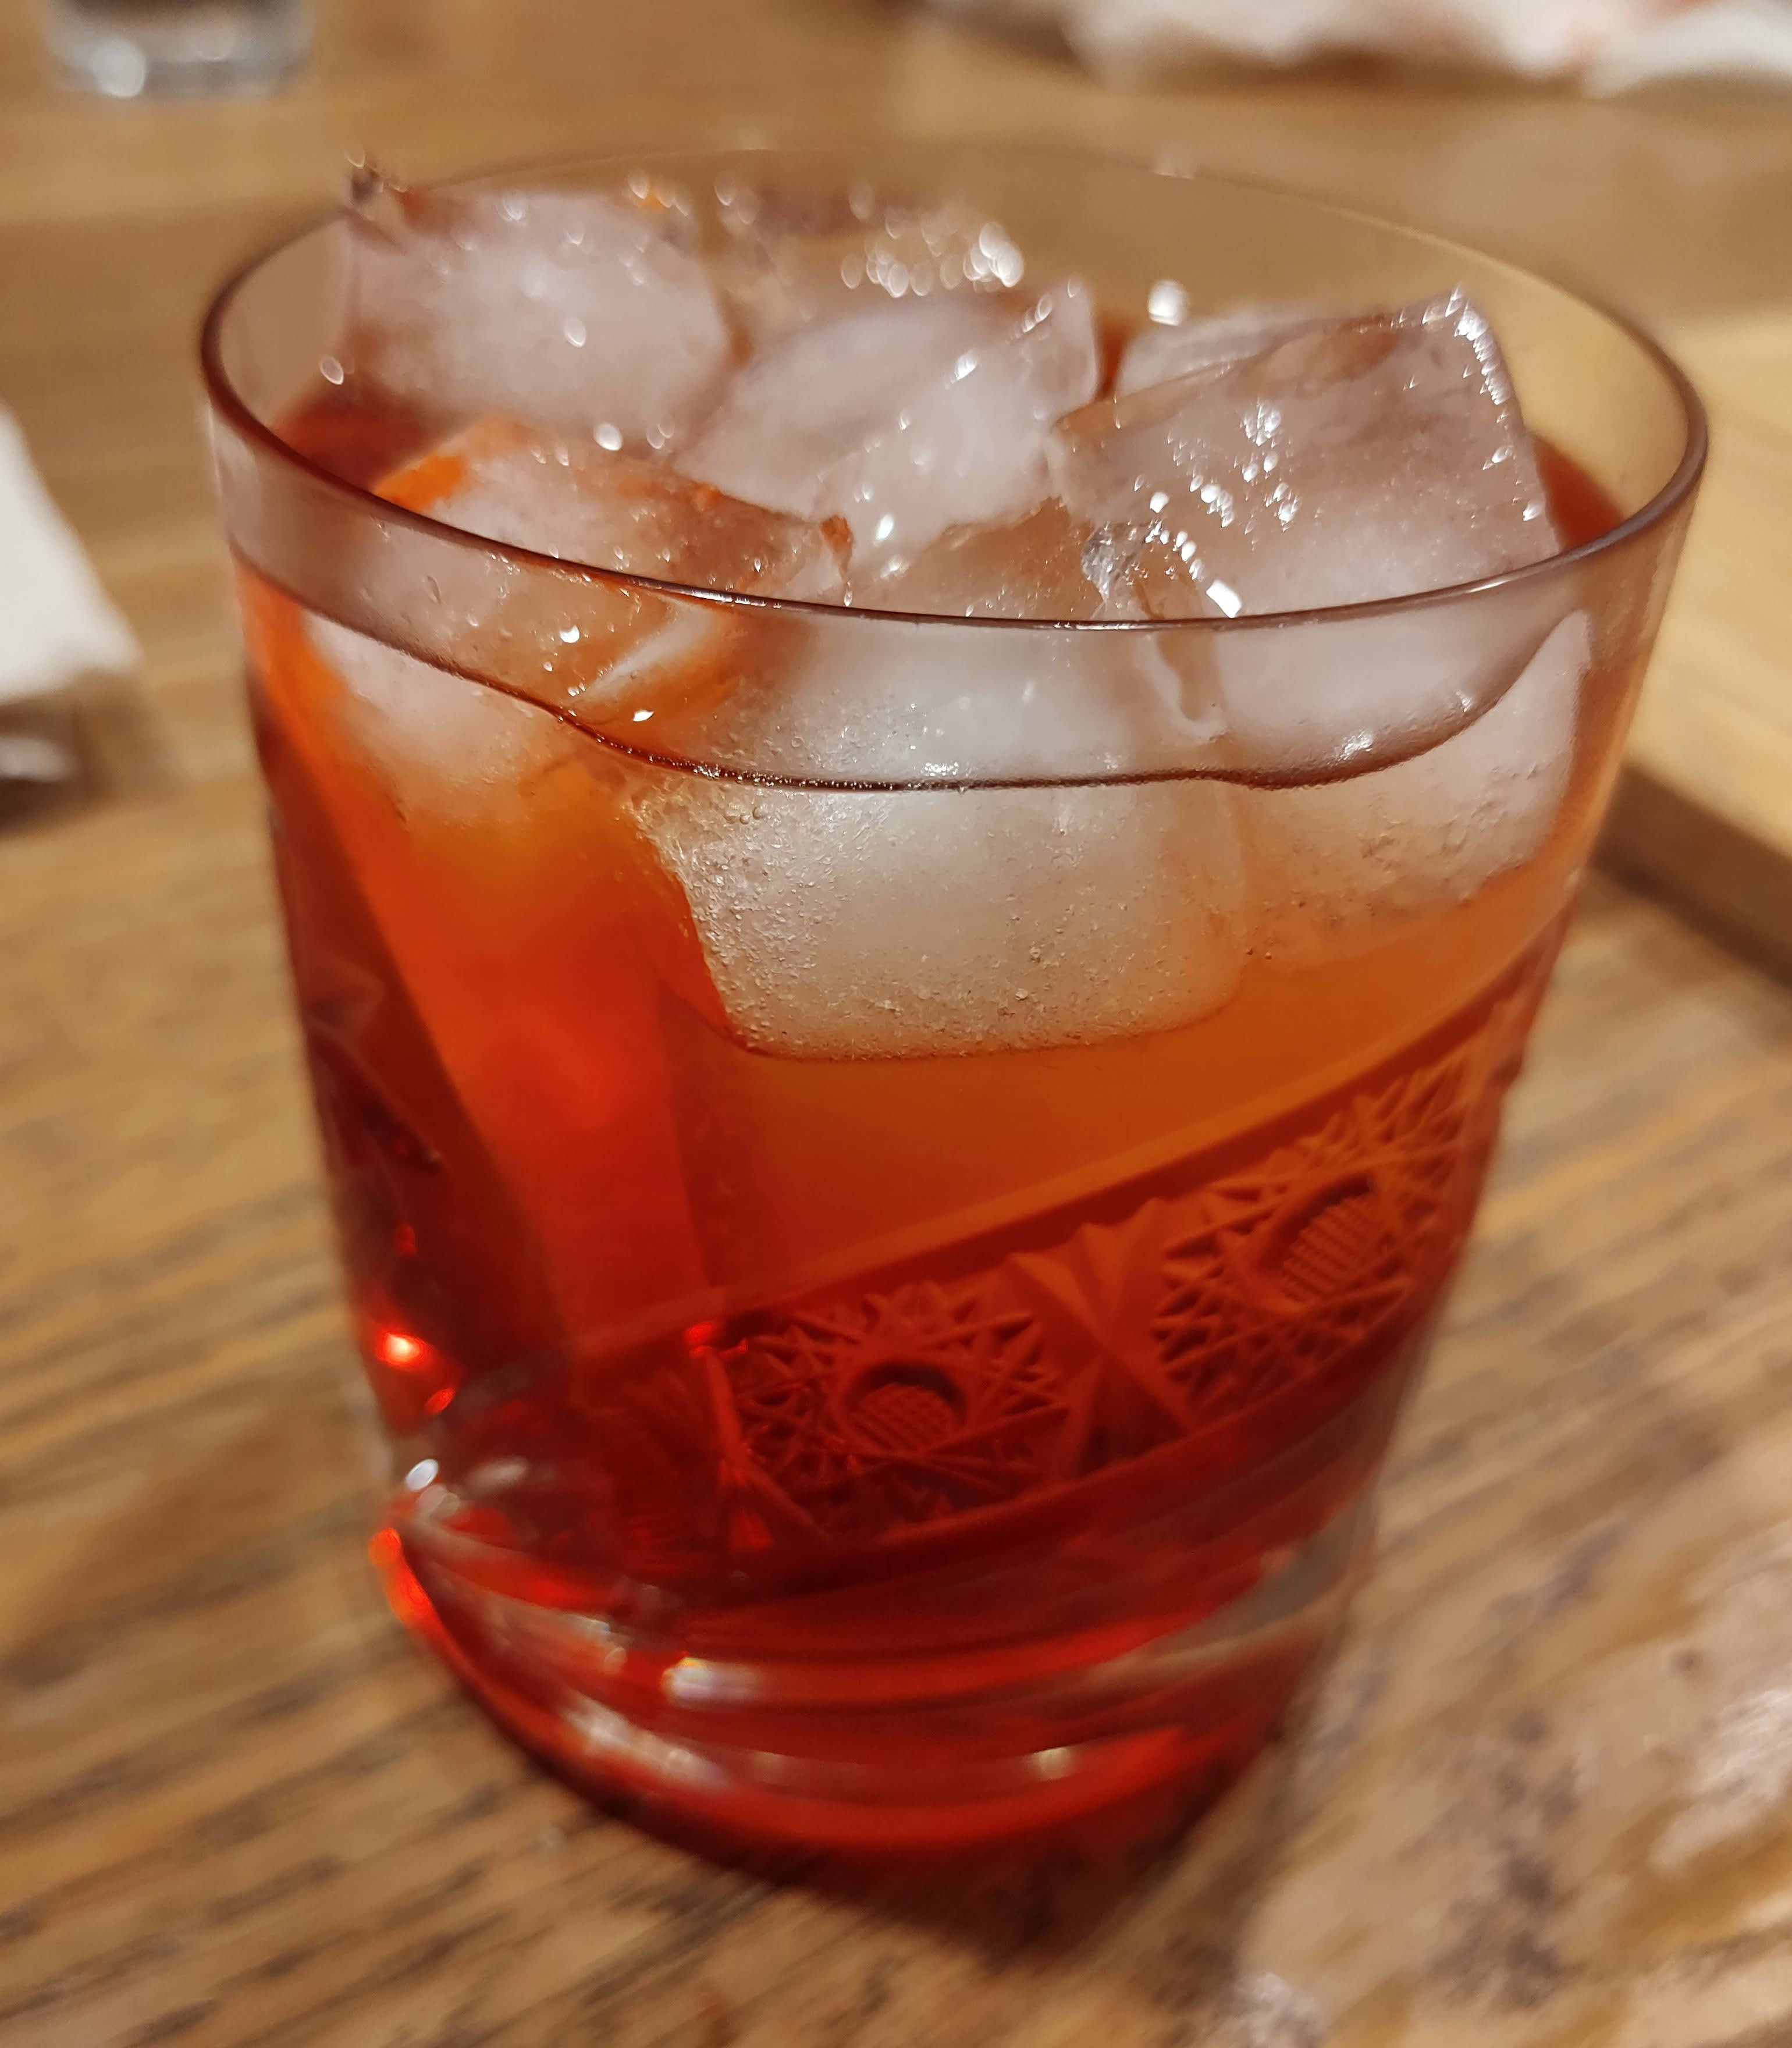
\includegraphics[width=5cm]{img/negroni.jpg}
\end{center}
%\showit[1.25in]{img/negroni.jpg}{This is a picture}







\newpage
\part{Indici}
\printindex
\end{document}
